%! TeX program = lualatex
\documentclass{article} 

\title{Wielomian Alexandera}
\author{Weronika Jakimowicz}
\date{}

\usepackage{tikz}
\usetikzlibrary{cd, patterns, patterns.meta, decorations.pathmorphing, calc, matrix, positioning, arrows, arrows.meta}
\usetikzlibrary{spath3, hobby, knots, braids}

\usepackage{graphicx}

\usepackage[utf8]{inputenc}
\usepackage[T1]{fontenc}

\usepackage{fontspec}

\usepackage[default]{cantarell}


\usepackage[
  a4paper,
  total={170mm, 247mm},
  left=20mm,
  top=25mm,
  % showframe
]{geometry}

\usepackage[skip=3mm]{parskip}
\renewcommand{\baselinestretch}{1.2}
\selectfont


\usepackage{amsfonts}
\usepackage{amsmath}
\usepackage{amssymb}

\usepackage{mathastext}

\DeclareMathOperator{\Spec}{Spec}

\usepackage{xcolor}

\definecolor{rosewater}{HTML}{dc8a78}
\definecolor{flamingo}{HTML}{dd7878}
\definecolor{pink}{HTML}{ea76cb}
\definecolor{mauve}{HTML}{8839ef}
\definecolor{red}{HTML}{d20f39}
\definecolor{maroon}{HTML}{e64553}
\definecolor{peach}{HTML}{fe640b}
\definecolor{yellow}{HTML}{df8e1d}
\definecolor{green}{HTML}{40a02b}
\definecolor{teal}{HTML}{179299}
\definecolor{sky}{HTML}{04a5e5}
\definecolor{sapphire}{HTML}{209fb5}
\definecolor{blue}{HTML}{1e66f5}
\definecolor{lavender}{HTML}{7287fd}
\definecolor{subtext2}{HTML}{4c4f69}
\definecolor{subtext1}{HTML}{5c5f77}
\definecolor{subtext0}{HTML}{6c6f85}
\definecolor{overlay2}{HTML}{7c7f93}
\definecolor{overlay1}{HTML}{8c8fa1}
\definecolor{overlay0}{HTML}{9ca0b0}

\definecolor{text}{HTML}{000000}
\color{text}

\makeatletter 
\let\htitle\@title
\let\fauthor\@author
\makeatother

\usepackage{fancyhdr}

\fancyfoot[CE, CO]{}
\fancyfoot[LE, RO]{\color{overlay2}\thepage}

\fancyhead[RE, LO]{$ \quad $\color{subtext1}\fauthor $ \quad $}
\fancyhead[LE, RO]{$ \quad $\color{green!40!subtext2}\bfseries\htitle $ \quad $}

\fancypagestyle{plain}{%
  \fancyhf{}%
  \fancyfoot[CE, CO]{}
  \fancyfoot[LE, RO]{\color{overlay2}\thepage}

  \fancyhead[RE, LO]{$ \quad $\color{subtext1}\fauthor $ \quad $}
  \fancyhead[LE, RO]{$ \quad $\color{green!40!subtext2}\bfseries\htitle $ \quad $}
}
\usepackage{dashrule}

\renewcommand{\headrule}{\color{overlay0}\hdashrule[.5ex]{\headwidth}{1pt}{1pt}}

\pagestyle{fancy}

\usepackage{titlesec}

\titleformat{\chapter}[block]{\bfseries\Huge}{\color{green!40!subtext2}\filright\Huge\thechapter.}{1ex}{\color{green!40!subtext2}\Huge\filright}

\titlespacing*{\chapter}{0pt}{0pt}{20pt}

\usepackage{amsthm}
\usepackage{thmtools}
\usepackage{tcolorbox}

% \RequirePackage[framemethod=TikZ]{mdframed}

\tcbuselibrary{theorems}
\tcbuselibrary{breakable}
\tcbuselibrary{skins}

\tcbset{greenTHM/.style={
    fonttitle = \bfseries\large,
    coltitle = green!50!black,
    description color = green!50!black, 
    description font = \bfseries\large,
    colbacktitle = white, %green!40!black!75,
    breakable, 
    enhanced,
    attach boxed title to top left = {
      xshift=0.5cm, 
      yshift=-\tcboxedtitleheight/2
    },
    boxed title style = {
      boxrule=0pt,
      colframe=white
    },
    top=6mm,
    bottom=4mm,
    colback=white,
    frame hidden,
    borderline={1pt}{0pt}{green!40},
    arc=0mm,
    after skip=5mm,
    before skip=5mm
  }
}

\tcbset{orangeTHM/.style={
    fonttitle = \bfseries\large,
    coltitle = orange!60!black,
    description color = orange!60!black, 
    description font = \bfseries\large,
    colbacktitle = white, %green!40!black!75,
    breakable, 
    enhanced,
    attach boxed title to top left = {
      xshift=0.5cm, 
      yshift=-\tcboxedtitleheight/2
    },
    boxed title style = {
      boxrule=0pt,
      colframe=white
    },
    top=6mm,
    bottom=4mm,
    colback=white,
    frame hidden,
    borderline={1pt}{0pt}{orange!40}, 
    arc=0mm,
    before skip=5mm,
    after skip=5mm
  }
}

\NewTcbTheorem[
  auto counter, 
  % number within=chapter
  number within=section
]{definition}{Definition}{greenTHM}{def} 

\NewTcbTheorem[
  use counter from=definition
]{theorem}{Theorem}{orangeTHM}{th}

\NewTcbTheorem[
  use counter from=definition
]{proposition}{Proposition}{orangeTHM}{prop}


\usepackage{svg}

\renewenvironment{proof}{{\bfseries\color{green!60!black} Dowód}$ $\newline}{
  \begin{flushright} \includesvg[width=4mm]{../../../../duck.svg} \end{flushright}$ $\newline
}

\usepackage{soul}

\sethlcolor{green!15}

\makeatletter
%\font\SOUL@tt="LMMono10-Regular"
\setbox\z@\hbox{\SOUL@tt-}
\SOUL@ttwidth\wd\z@ %
\makeatother

\newcommand{\buff}[1]{
  {\bfseries\color{green}#1}
}

\usepackage{enumitem}
 

\begin{document}

\maketitle 

\section{Macierze}

\section{Węzły - definicje}

\begin{definition}{Węzeł}{}
Węzeł to sposób ułożenia okręgu w przestrzeni $3$ wymiarowej tak, by dało się spojrzeć na niego z góry i w każdym punkcie zobaczyć nie więcej niż dwa punkty z okręgu. 

Tzn. nie możemy mieć $3$ sznurków z węzła przecinających się w jednym miejscu.
\end{definition}

\begin{center}
  \includegraphics[width=10cm]{knot_4_1.png}

  Węzeł zwykle używany do robienia guzełków, matematycznie znany jako $4_1$, bo ma $4$ skrzyżowania.
\end{center}

Zauważmy, że ten węzeł można łatwo zmienić tak, by wyglądał na węzeł o $5$ skrzyżowaniach (na tablicy narysuję pierwszy ruch na którejś nitce). W gruncie rzeczy taki ruch nie zmienia nam węzła - jak pociągniemy za sznurówki to nadal dostaniemy guziołek z $4_1$.

Matematycznie, dwa węzły są \emph{równoważne}, czyli takie same, jeśli można jeden w drugi przekształcić za pomocą tak zwanych \textbf{ruchów Reidemeistera}.

\begin{center}
  \includegraphics[width=10cm]{reidemeister_moves.png}

  Ruchy Reidemeistera, można wykonywać je w obie strony.
\end{center}

{\centering\bfseries\large\color{green!70!black}
  Pojawia się pytanie, jak szybko sprawdzić, czy dwa skomplikowane węzły są tym samym?
}

Weźmy na przykład dwa węzły jak niżej, jeden o $6$ skrzyżowaniach, a drugi o $9$.

\begin{center}
  \includegraphics[width=8cm]{knot_6_1.png}
  \includegraphics[width=8cm]{knot_9_46.png}

  Po lewej jest węzeł $6_1$ a po prawej $9_{46}$.
\end{center}

\section{Orientacja węzła i diagramu}

Na okręgu możemy narysować strzałkę. Ta strzałka jest zachowywana, gdy robimy z okręgu węzeł.

\begin{definition}{Zorientowany węzeł}{}
  Węzeł z zaznaczoną strzałką nazwiemy węzłem zorientowanym.
\end{definition}

W zorientowanym diagramie zawsze mamy dwa rodzaje skrzyżowań:
\begin{center}
  \begin{tikzpicture}
    \draw[->, very thick] (0, 0)--(0, 3);
    \fill[white] (0, 1.5) circle (5pt);
    \draw[->, very thick] (-1.5, 1.5)--(1.5, 1.5);

    \node at (0, -.5) {\Large\bfseries+};


    \draw[->, very thick] (4.5, 0)--(4.5, 3);
    \fill[white] (4.5, 1.5) circle (5pt);
    \draw[<-, very thick] (3, 1.5)--(6, 1.5);

    \node at (4.5, -.5) {\Large\bfseries-};
  \end{tikzpicture}
\end{center}
Nazwiemy je $+$ i $-$ tak jak na obrazku. Które skrzyżowanie jest $+$ nie ma znaczenia - ważne jest aby trzymać się cały czas jednej konwencji.

W zorientowanych diagramach węzłów mamy o jeden ruch Reidemeistera więcej. Ruch 1 z obrazka wyżej musi mieć dwa warianty - dla skrzyżowania $+$ i dla skrzyżowania $-$.

\begin{center}
  \includegraphics[width=10cm]{oriented_reidemeister.png}
\end{center}

Zdarza się, że jedna orientacja węzła nie jest równoważna przeciwnej orientacji tego samego węzła. To nas jednak nie interesuje, bo niezmiennik węzła, jakim się dzisiaj zajmiemy rozróżnia węzły, a nie ich orientacje. Istnieją inne niezmienniki, które jednak zwracają na to uwagę, np. wielomian Jonesa.

\section{Kolorowanie węzłów}

Ściśle rzecz biorąc, węzłów nigdy nie kolorujemy - robimy to z ich diagramami. W diagramach zawsze skrzyżowania będą nam mówić, czy kolorowanie jest sensowne, czy też nie. Tym, czemu przypisujemy barwy może być obszar odgrodzony przez kawałek sznurka lub fragment nitki od jednego skrzyżowania do drugiego. Alexander w swojej pracy zajmował się tym pierwszym sposobem, jednak teraz króluje ten drugi sposób. Jest to związane z innym, o wiele trudniejszym i dokładniejszym niezmiennikiem węzła (grupa węzła).

\begin{center}
  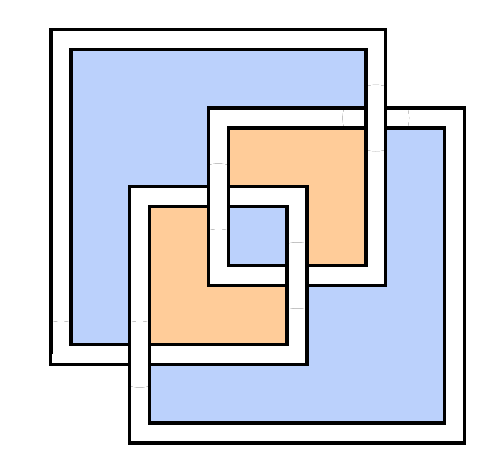
\begin{tikzpicture}
    \filldraw[fill=blue!30] (0, -4)--(0,0)--(4, 0)--(4, -1)--(2, -1)--(2, -2)--(1, -2)--(1, -4)--(0, -4);
    \filldraw[fill=orange!40] (4, -1)--(2, -1)--(2, -2)--(3, -2)--(3, -3)--(4, -3)--(4, -1);
    \filldraw[fill=orange!40] (1, -4)--(3, -4)--(3, -3)--(2, -3)--(2, -2)--(1, -2)--(1, -4);
    \filldraw[fill=blue!30] (2, -3)--(3, -3)--(3, -2)--(2, -2)--(2, -3);
    \filldraw[fill=blue!30] (1, -4)--(1, -5)--(5, -5)--(5, -1)--(4, -1)--(4, -3)--(3, -3)--(3, -3)--(3, -4)--(1, -4);
    \begin{knot}[ 
      consider self intersections,
      ignore endpoint intersections=false,
      clip width=2,
      % draft mode=crossings,
      background color=white,
      only when rendering/.style={
        draw=black,
        double=white,
        double distance=6pt, 
        %line cap=round
      },
      flip crossing=2,
      %flip crossing=5,
      flip crossing=4
      ]
      \strand[very thick] 
        (0, -4) to 
        (0, 0) to 
        (4, 0) to 
        (4, -3) to 
        (2, -3) to 
        (2, -1) to 
        (4, -1) to 
        (5, -1) to 
        (5, -5) to 
        (1, -5) to 
        (1, -2) to 
        (3, -2) to 
        (3, -4) to 
        (0, -4);
    \end{knot}
    \fill[white] (-0.1, -4.09) rectangle (0.18, -3.9);
    \draw[very thick](-0.13, -4)--(-0.13, -4.13)--(0.1, -4.13);


  \end{tikzpicture}

  Przykład kolorowania obszarów węzła.
\end{center}

\begin{definition}{Kolorowanie węzła}{}
  Ponumerujmy łuczki/segmenty węzła, czyli kawałki okręgu między dwoma kolejnymi skrzyżowaniami - będą one $l_1,..., l_n$. Zróbmy to samo ze skrzyżowaniami, które będziemy nazywać $x_1,..., x_n$ i będziemy je traktować jako maszynki, które przyjmują kolory $3$ łuczków: \textbf{górny, wchodzący i wychodzący}, i mówią, czy kolorowanie jest dobre (wartość $0$) czy nie (wartość różna od $0$).

  {\bfseries\color{green}Kolorowaniem nazwiemy przyporządkowanie łuczkom kolorów (liczb całkowitych) w taki sposób, że każde skrzyżowanie zwraca nam liczbę $\boldsymbol0$.}
\end{definition}

Każdy artysta ma inną paletę, więc maszynki którymi są skrzyżowania mogą działać na wiele sposobów. My dzisiaj będziemy się zajmować dwoma konkretnymi paletami, które działają jak funkcje:
\begin{align*}
  x_i^+(u, i, o)=(1-t)u+ti-o \quad & \quad x_i^-(u,i,o)=(1-t^{-1})u+t^{-1}i-o\\ 
  x_i^+(u,i,o)=2u-i-o \quad & \quad x_i^-(u,i,o)=2u-i-o
\end{align*}
Zauważmy, że dolny wiersz powstał z górnego przez podstawienie $t\mapsto -1$.

Zaczniemy od działania na drugiej palecie z racji, że jest prostsza. Możemy ją zapisać w postaci \emph{macierzy}, chociaż nie kwadratowej:
$$\begin{bmatrix}2&-1&-1\end{bmatrix}\begin{bmatrix}u\\i\\o\end{bmatrix}$$
Mając kilka skrzyżowań możemy zbudować z takich poziomych paseczków większą, kwadratową macierz, którą będziemy nakładać na kolumn zawierające interesujące nas kolory łuczków. Lepiej pokazać to na przykładzie.

\begin{center}
  \begin{tikzpicture}
    \begin{knot}[
      consider self intersections, 
      clip width = 20pt, 
      % draft mode=crossings, 
      flip crossing=2
      ] 
      \strand[->, thick] (90:2) to[out=0, in=-60, looseness=2]
      (210:2) to[out=120, in=60, looseness=2]
      (-30:2) to[out=-120, in=180, looseness=2] 
      (90:2);
    \end{knot}

    \begin{scope}[shift={(7, 1.8)}]
    \matrix (m) [
      matrix of nodes, 
      left delimiter = {[}, 
      right delimiter={]},
      column sep=5mm
    ]
      {
              2  & -1 & 1  \\
              -1 & 1  & 2  \\
              1  & 2  & -1 \\
      };
         
    \draw[red, thick, dashed] (m-1-1.north west) rectangle (m-2-2.south east);
    \node at ($(m-1-1)!0.5!(m-1-2)+(0, .7)$) {$\color{red}1$};

    \draw[green, thick, dashed] (m-2-2.north west) rectangle (m-3-3.south east);
    \node at ($(m-3-2)!0.5!(m-3-3)+(0, -0.7)$) {$\color{green}-5$};
      \node at ($(m-2-1.west)+(-1.8, 0)$) {$P_1(D)=$};
    \end{scope}
    
    \begin{scope}[shift={(7, -1.8)}]
      \matrix (m) [
        matrix of nodes, 
        left delimiter = {[}, 
        right delimiter={]},
        column sep=5mm
      ]
        {
                2  & -1 & -1  \\
                -1 & -1  & 2  \\
                -1  & 2  & -1 \\
        };
           
      \draw[red, thick, dashed] (m-1-1.north west) rectangle (m-2-2.south east);
      \node at ($(m-1-1)!0.5!(m-1-2)+(0, .7)$) {$\color{red}-3$};

      \draw[green, thick, dashed] (m-2-2.north west) rectangle (m-3-3.south east);
      \node at ($(m-3-2)!0.5!(m-3-3)+(0, -0.7)$) {$\color{green}-3$};
      \node at ($(m-2-1.west)+(-1.8, 0)$) {$P_2(D)=$};
    \end{scope}
    % \begin{scope}[shift={(7, 2.5)}]
    %   \matrix (m) [
    %     matrix of nodes, 
    %     left delimiter = {[}, 
    %     right delimiter={]},
    %     column sep=5mm
    %   ]
    %     {
    %       0  & 2 & 1 & -1  \\
    %       0  & -1 & 2  & 1  \\
    %       1  & 0  & -1  & 2 \\
    %       1 & 1 & 0 & 0 \\
    %     };
    %
    %   \draw[red, thick, dashed] (m-1-1.north west) rectangle (m-3-3.south east);
    %   \node at ($(m-1-1)!0.5!(m-1-3)+(0, .7)$) {$\color{red}5$};
    %
    %   \draw[green, thick, dashed] (m-2-2.north west) rectangle (m-4-4.south east);
    %   \node at ($(m-4-2)!0.5!(m-4-4)+(0, -0.7)$) {$\color{green}5$};
    %
    %   \draw[blue, thick, dashed] ($(m-1-2.north west)+(-0.01, 0.1)$) rectangle ($(m-3-4.south east)+(0.1, 0.1)$);
    %   \node at ($(m-1-2)!0.5!(m-1-4)+(0, 0.7)$) {$\color{blue}11$};
    %
    %   \node at ($(m-2-1.west)+(-1.8, 0)$) {$P_1(D)=$};
    % \end{scope}

  \end{tikzpicture}
\end{center}

\end{document}
